\documentclass[12pt]{article}
\usepackage{amsmath}
\usepackage{amssymb}
\usepackage[letterpaper,top=0.8in,bottom=1in,left=0.75in,right=0.75in,centering]{geometry}
\usepackage{fancyhdr}
\usepackage{enumerate}
%\usepackage{lastpage}
\usepackage{multicol}
\usepackage{graphicx}
\usepackage{tikz}
\usetikzlibrary{calc, positioning, decorations.pathmorphing}

\reversemarginpar

\pagestyle{fancy}
\chead{Math 1565 Tutorial \#8 Solutions}
%\cfoot{}
%\lhead{Math 1560}\chead{Test \# 1}\rhead{May 18th, 2017}
%\rfoot{Total: 10 points}
%\chead{{\bf Name:}}
\newcommand{\points}[1]{\marginpar{\hspace{24pt}[#1]}}
\newcommand{\skipline}{\vspace{12pt}}
\renewcommand{\headrulewidth}{0in}
\headheight 30pt

\newcommand{\di}{\displaystyle}
\newcommand{\abs}[1]{\lvert #1\rvert}
\newcommand{\len}[1]{\lVert #1\rVert}
\renewcommand{\i}{\mathbf{i}}
\renewcommand{\j}{\mathbf{j}}
\renewcommand{\k}{\mathbf{k}}
\newcommand{\R}{\mathbb{R}}
\newcommand{\aaa}{\mathbf{a}}
\newcommand{\bbb}{\mathbf{b}}
\newcommand{\ccc}{\mathbf{c}}
\newcommand{\dotp}{\boldsymbol{\cdot}}
\newcommand{\bbm}{\begin{bmatrix}}
\newcommand{\ebm}{\end{bmatrix}}                   
                  
\begin{document}


\author{Instructor: Sean Fitzpatrick}



%\thispagestyle{empty}

\begin{enumerate}
  \item Find the absolute maximum and minimum of $f(x)=3x^{2/3}-2x$ on $[-1,2]$. \points{4} 
 
 
 
\medskip

\textbf{Solution:} We first check the endpoints:
\[
f(-1) = 3(1)-2(-1)=5, \text{ and } f(2) = 3(2^{2/3})-2(2) \approx 0.762
\]
Next, we find
\[
f'(x) = 2x^{-1/3}-2 = \frac{2(1-x^{1/3})}{x^{1/3}},
\]
so $f'(x)=0$ when $x=1$, and $f'(x)$ is undefined when $x=0$. Both points are in the domain of $f$ (and the given interval), so both are critical numbers. The critical values are
\[
f(0) = 0 \text{ and } f(1) = 1.
\]
Comparing values, we see that the absolute minimum is $f(0)=0$, and the absolute maximum is $f(-1)=5$.
 
 \medskip
  
 \item Use the Mean Value Theorem to show that for any $a,b\in\R$,\points{2}
 \[
 \abs{\sin(b)-\sin(a)}\leq \abs{b-a}.
 \]
 

 \medskip
 
\textbf{Solution:} Consider $f(x)=\sin(x)$, and choose any two real numbers $a$ and $b$. We can assume $a<b$ since the result holds when $a=b$ (since $0\leq 0$), and if $a>b$ we can simply reverse the roles of $a$ and $b$. We know that $f$ is continuous on $[a,b]$ and differentiable on $(a,b)$, so by the Mean Value Theorem, there exists some $c\in (a,b)$ such that 
 \[
 \sin(b)-\sin(a)=\cos(c)(b-a),
 \]
 using the fact that $f'(x)=\cos(x)$. If we take the absolute value of both sides of this equation, we get
 \[
 \abs{\sin(b)-\sin(a)}=\abs{\cos(c)}\abs{b-a} \leq 1\abs{b-a},
 \]
 since $\abs{\cos(c)}\leq 1$, which is what we needed to show.
 
 \medskip
 
 \item Find and classify the critical points of $f(x)=e^x\sin(x)$ for $x\in [0,2\pi]$\points{4}
 
 \medskip
 
 \textbf{Solution:} Using the product rule, we find
 \[
 f'(x) = e^x\sin(x)+e^x\cos(x)=e^x(\sin(x)+\cos(x)).
 \]
 Since $e^x\neq 0$ for all $x\in \R$, the critical points must occur when $\sin(x)+\cos(x)=0$, or equivalently, when $\tan(x)=-1$.

 For $x\in [0,2\pi]$, this is satisfied when $x=3\pi/4$ and $x=7\pi/4$. Choosing appropriate test values ($0$, $\pi$, and $2\pi$ are good choices), we find that the sign diagram is given by
 \begin{center}
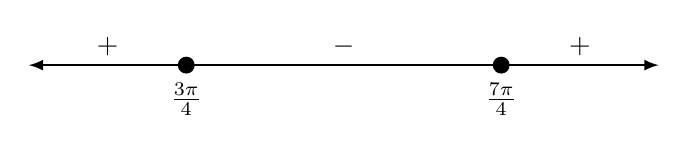
\begin{tikzpicture}[>=latex]
  \draw [thick, <->] (-4,0) -- (4,0);
  \draw [fill] (-2,0) circle [radius =.1];
  \draw [fill] (2,0) circle [radius =.1];
  \node at (-3,0) [above] {$+$};
  \node at (0,0) [above] {$-$};
  \node at (3,0) [above] {$+$};
  \node at (-2,-0.1) [below] {$\frac{3\pi}{4}$};
  \node at (2,-0.1) [below] {$\frac{7\pi}{4}$};
  \end{tikzpicture}
\end{center}
Using the First Derivative Test, we see that $\left(\dfrac{3\pi}{4},\dfrac{1}{\sqrt{2}}e^{3\pi/4}\right)$ is a local maximum, and $\left(\dfrac{7\pi}{4},-\dfrac{1}{\sqrt{2}}e^{7\pi/4}\right)$ is a local minimum.
\end{enumerate}
\end{document}